\documentclass[a4paper,12pt]{book}
\usepackage[utf8]{inputenc}
\usepackage[spanish]{babel}
\usepackage[Glenn]{fncychap}

\usepackage{amsmath, amssymb, geometry, graphicx, fancyhdr, hyperref, titlesec, titling, tocloft, tcolorbox, booktabs, appendix, listings, xcolor, caption, subcaption}

\renewcommand{\sectionmark}[1]{\markboth{#1}{}}
\renewcommand{\subsectionmark}[1]{\markright{#1}}

%\graphicspath{{../graphs/}}

\geometry{margin=2.5cm}
\setlength{\parskip}{1em}
\setlength{\parindent}{0em}

\pagestyle{fancy}
\fancyhf{}
\fancyhead[L]{
\includegraphics[width=1.5cm]{./TeX_files/logo.png}}
\fancyhead[C]{}
\fancyhead[R]{\nouppercase{\leftmark}}

\fancyfoot[C]{\thepage}

\hypersetup{
	colorlinks=true,
	linkcolor=blue,
	urlcolor=blue,
	pdftitle={Proyecto Optimización},
	pdfauthor={Simón Valdés Oliva},
}






\begin{document}

\begin{titlepage}
	\begin{center}
		\vspace*{1cm}

		
\includegraphics[width=4cm]{./TeX_files/logo.png}

		\vspace{1.5cm}

		{\Huge\bfseries Proyecto: Optimización del uso del Hospital Regional Villa Zarcillo\par}

		\vspace{1cm}

		\rule{\textwidth}{0.4pt}

		\vspace{0.5cm}

		{\Large ING200 -- Optimización\\[0.3cm]}
		{\large Prof. Jorge Acuña, PhD.}

		\vspace{0.5cm}

		\rule{\textwidth}{0.4pt}

		\vspace{2cm}

		{\Large
			\begin{tabular}{c}
				Simón Valdés Oliva \\[0.3cm]
				Vicente Díaz
			\end{tabular}
		}

		\vfill

		{\large Universidad Adolfo Ibáñez\\[0.2cm]
		Viña del Mar\\[0.5cm]
		\today}

	\end{center}
\end{titlepage}
\newpage
\tableofcontents


\newpage

\chapter{Introducción}
 	El Hospital Regional de Villa Zarcillo, al igual como otros hospitales del país, se encuentra
 	en una situación crítica respecto a las cirugías electivas dada la suspensión de estas en el
 	periodo de pandemia.
 	
 	Debido a esto, desde el Gobierno, se ha tomado la decisión de habilitar un contingente de
 	salud, conformado por pabellones móviles junto a sus respectivos equipos de salud a fin de
 	recorrer distintas ciudades del país realizando operaciones electivas a fin de descongestionar
 	los hospitales.
 	
 	Durante la semana del 6 de julio, desde el día lunes hasta el día viernes, el contingente de
 	salud llegará a Villa Zarcillo. Debido a esto, en conjunto con el hospital, deben determinar
 	las operaciones a realizar junto con la respectiva asignación de pabellones.
 	
 	Para definir el plan de las operaciones a realizar, se tienen las siguientes consideraciones:
 	\begin{itemize}
 		\item Del conjunto de operaciones del Hospital, no todas deben ser realizadas. 
 		\item Cada operación tiene un tipo de especialidad, un tiempo de realización y un costo asociado para el Estado.
 		\item Existe un conjunto de pabellones. En cada pabellón, se pueden realizar solamente ciertos tipos de operaciones, por ende, solo se puede realizar una operación en un pabellón que lo permita.
 		\item Cada operación que inicia un día debe ser completada ese mismo día. Además, cada pabellón puede tener una operación a la vez y los horarios son de 10:00 a 20:00.
 		\item Entre cada operación, debe existir una limpieza total de 1 hora. Al final del día, los pabellones se limpian luego de la última operación, no importando si la limpieza sobrepasa las 20:00.
 		\item Se posee un presupuesto de \textbf{\$100.000.000}.
 	\end{itemize}
 	
 	El objetivo de este informe es optimizar el funcionamiento del hospital, máximizando la cantidad de pacientes atendidos, el uso de los pabellones, siguiendo las restricciones dadas.
 	
 	
 	\chapter{Desarrollo}
 	\section{Modelado}
 	A partir de las consideraciones, diseñamos el siguiente modelo de optimización: 
 	\paragraph{Variables:} $$X_{i,j,k} = \begin{cases}
 		1 \text{ si la operación $i$ se realiza en el pabellón $j$ el día $k$} \\
 		0 \text{ si no se realiza}
 	\end{cases}$$
 	
 	$$c_i = \text{Costo en pesos de la operación } i $$
 	$$t_i = \text{Tiempo en horas de la operación } i $$
 	
 	$$p_{i,j}= \begin{cases}
 		1 \text{ si la operación $i$ se puede realizar en el pabellón $j$} \\
 		0 \text{ si no se puede}
 	\end{cases}
 		$$
 		
 
 	\paragraph{Conjuntos:}\textcolor{white}{newline}
 	
	Operaciones: 
 	$$i \in I = [1,100]$$
 	Pabellones:
 	$$j \in J = [1,5]$$
 	Días:
 	$$k \in K = [1,5]$$
 	
 	\paragraph{Restricciones}\textcolor{white}{newline}
 	
 	\textbf{1. Presupuesto:} La suma de todas las operaciones a realizar en multiplicadas por el costo de su respectiva operación debe ser menor al presupuesto de \$100.000.000.
 	$$\sum_{i\in I} \sum_{j \in J} \sum_{k \in K} X_{i,j,k} C_i \leq 100.000.000$$
 	
 	\textbf{2. No se repiten las operaciones: }Para todas las operaciones, la suma de las operaciones de un cierto tipo debe ser menor o igual a 1 para todos los pabellones y días.
 	$$\sum_{j \in J} \sum_{k \in K} X_{i,j,k} \leq 1, \forall i \in I$$
 	
 	\textbf{3. Tiempo diario disponible: }El tiempo disponible son 10 horas al día, por cada pabellón, además hay que considerar la hora de limpieza post operación, por lo que cada operación dura $t_i + 1$ horas en total. Cómo la última limpieza (posterior a las 20:00) no es considerada en horas de limpieza, lo restamos a nuestra restricción, y como esta debe ser menor o igual a las 10 horas disponibles, sumamos 1 a ambas partes para simplificar.
 	$$\sum_{i \in I} (t_i + 1)X_{i,j,k} \leq 11, \forall j \in J, k \in K$$
 	
 	\textbf{4. Compatibilidad:}Solo se puede asignar una operación a un pabellón si este admite ese tipo.\footnote{En el documento Jupyter no se usa esta restricción de forma explícita ya que se implementó una lista \texttt{combinaciones} que filtra previamente las tuplas válidas. Así, el modelo en Gurobi solo crea las variables de decisión para las operaciones y pabellones que son compatibles.}
 	$$X_{i,j,k} \leq P_{i,j}, \forall i \in I, j \in J, k \in K$$
 	
 	\paragraph{Función objetivo}
 	
	$$\max Z = \sum_{i \in I} \sum_{j \in J} \sum_{k \in K} X_{i,j,k}$$

 	
 	\paragraph{Naturaleza de las variables}
 	
 	$$X_{i,j,k} = \{0,1\} \forall i \in I, j \in J, k \in K$$
 	$$c_i \in \mathbb{R}^+, \forall i \in I$$
 	$$t_i \in \mathbb{Z}^+, \forall i \in I$$
 	
 	\section{Resolución}
 	Usando la librería de Python del software de optimización \textit{Gurobi}, resolivmos el modelo, el cuál nos indicó que el óptimo se encuentra en 58 asignaciones.
 	$$Z_1^* = 58$$
 	Luego, en base a ese número decidimos ir resolviendo modelos de manera secuencial para obtener los costos óptimos y el óptimo de uso de tiempo. Para ello, agregamos la restricción: 
 	
 	$$\sum_{i \in I} \sum_{j \in J} \sum_{k \in K} X_{i,j,k} = 58$$
 	
 	Y modificamos la función objetivo para minimizar el costo:
 	
 	$$\min C = \sum_{i\in I} \sum_{j \in J} \sum_{k \in K} X_{i,j,k} c_i$$
 	
	Al resolver el modelo, nos entrega un valor óptimo de \$97.802.912
	
	$$C^* = 97.802.912$$
	
	Luego, agregamos este valor como restricción, siguiendo la misma lógica anterior:
	
	$$\sum_{i\in I} \sum_{j \in J} \sum_{k \in K} X_{i,j,k} = 97.802.912$$
	
	Finalmente, modificamos la función objetivo para maximizar la suma de las horas asignadas:
	
	$$\max T = \sum_{i\in I} \sum_{j \in J} \sum_{k \in K} X_{i,j,k} t_i$$
	
	Obteniendo un valor óptimo de 134 horas de operaciones:
	$$T^* = 134$$
	
	Pudimos obtener la siguiente información sobre el costo y uso de las operaciones que el modelo eligió como óptimas:
	
	\begin{table}[htbp]
		\centering
		\caption{Costos y Utilización}
		\label{tab:resumen_general}
		\begin{tabular}{lc}
			\toprule
			\textbf{Indicador} & \textbf{Valor} \\
			\midrule
			Total de Operaciones Realizadas & 58 \\
			Costo Total Asociado & \$97.802.912 \\
			Utilización Promedio de Pabellones & 53,60\% \\
			\bottomrule
		\end{tabular}
	\end{table}
	\newpage
	También, pudimos obtener la distribución de operaciones por día:
	\begin{table}[htbp]
		\centering
		\caption{Distribución Diaria}
		\label{tab:operaciones_diarias}
		\begin{tabular}{cc}
			\toprule
			\textbf{Día} & \textbf{Cantidad de Operaciones} \\
			\midrule
			Día 1 & 11 \\
			Día 2 & 8 \\
			Día 3 & 12 \\
			Día 4 & 10 \\
			Día 5 & 17 \\
			\midrule
			\textbf{Total} & \textbf{58} \\
			\bottomrule
		\end{tabular}
	\end{table}
	Finalmente, pudimos hacer un análisis del tipo de operación, el número de operaciones por tipo y su porcentaje respecto al total, el costo asociado por tipo y el porcentaje del presupuesto que dicho tipo de operación ocupa.
	\begin{table}[htbp]
		\centering
		\caption{Tipos de operaciones}
		\label{tab:analisis_especialidad}
		\begin{tabular}{lcrrc}
			\toprule
			\textbf{Tipo de Operación} & \textbf{N° Ops.} & \textbf{\% Ops.} & \textbf{Costo Asociado} & \textbf{\% Presup.} \\
			\midrule
			Gástrica              & 12 & 20,69\% & \$23.540.589 & 24,07\% \\
			Traumatológica        & 8  & 13,79\% & \$16.150.372 & 16,51\% \\
			Ginecológica          & 8  & 13,79\% & \$13.960.515 & 14,27\% \\
			Vascular              & 2  & 3,45\%  & \$4.600.068  & 4,70\%  \\
			Dérmica               & 7  & 12,07\% & \$8.210.241  & 8,39\%  \\
			Urológica             & 2  & 3,45\%  & \$4.510.138  & 4,61\%  \\
			Oftalmológica         & 11 & 18,97\% & \$14.530.699 & 14,86\% \\
			Otorrinolaringológica & 8  & 13,79\% & \$12.300.290 & 12,58\% \\
			\midrule
			\textbf{Total}        & \textbf{58} & \textbf{100,00\%} & \textbf{\$97.802.912} & \textbf{100,00\%} \\
			\bottomrule
		\end{tabular}
	\end{table}
	\newline
	A su vez, pudimos graficar el cronograma diario con las asignaciones de operaciones correspondientes.
	
	
	\begin{figure}[htbp]
		\centering
		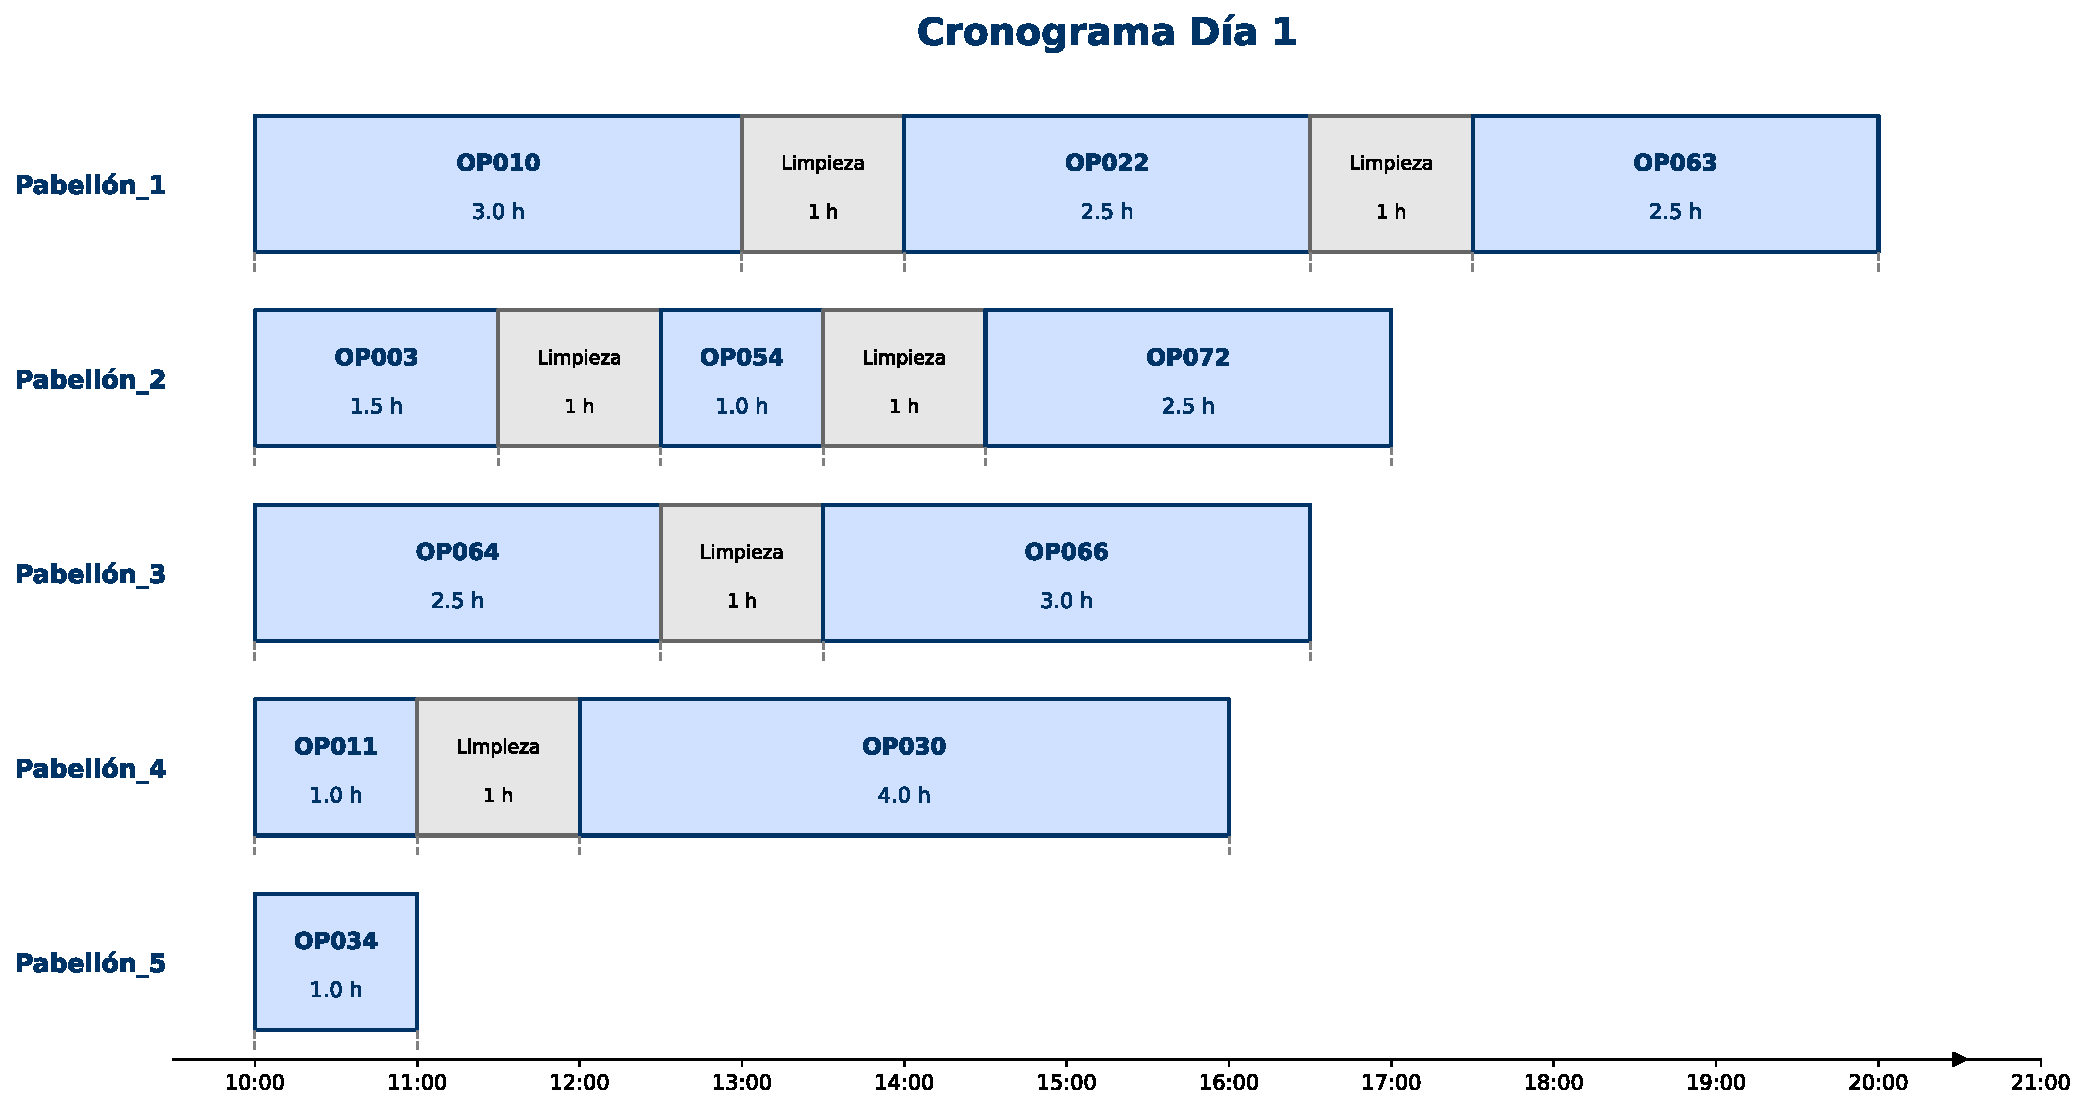
\includegraphics[width=0.8\textwidth]{./TeX_Files/graphs/Cronograma_Dia1.pdf}
		\caption{Cronograma con asignación de operaciones - Día 1.}
		\label{fig:cronograma_dia1}
	\end{figure}
	
	\begin{figure}[htbp]
		\centering
		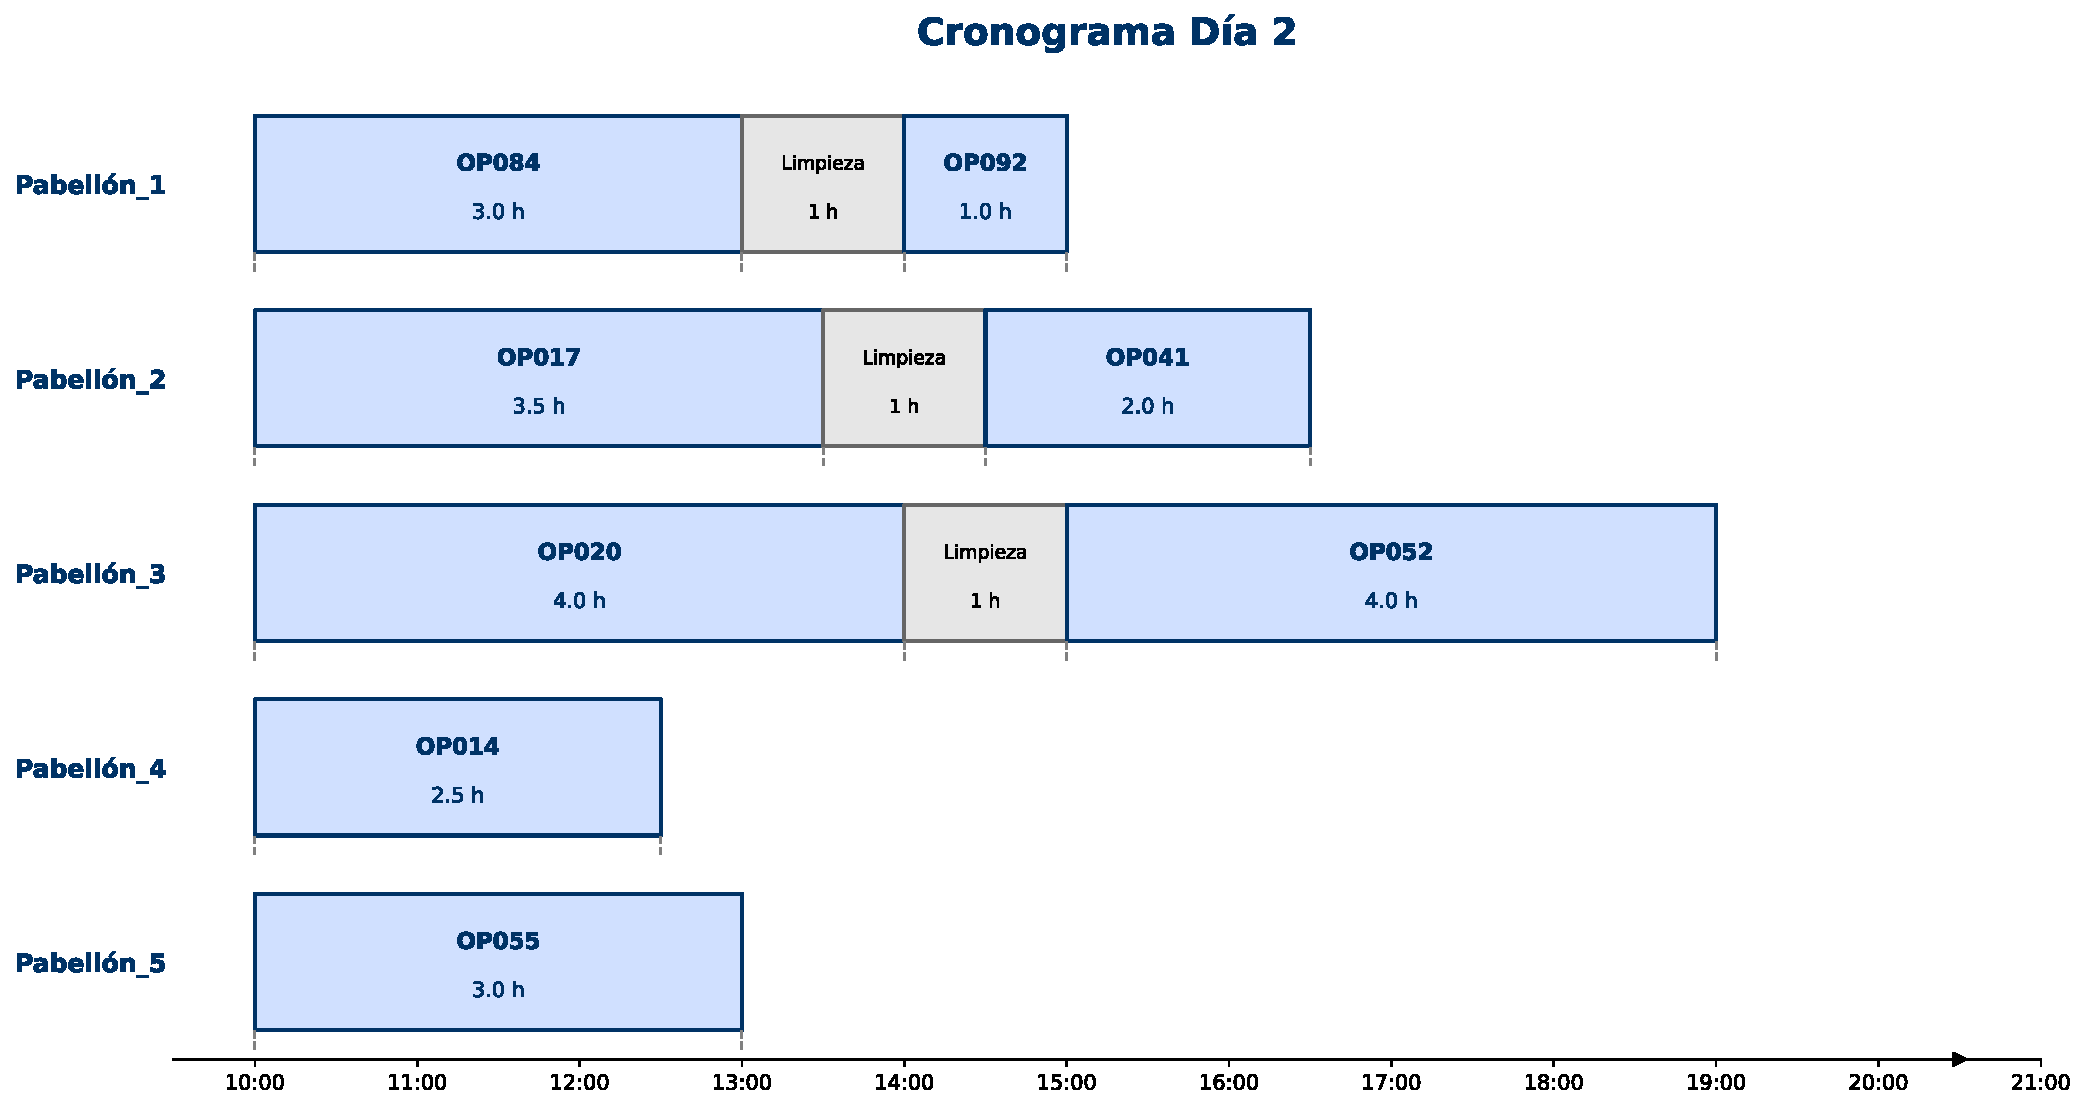
\includegraphics[width=0.8\textwidth]{./TeX_Files/graphs/Cronograma_Dia2.pdf}
		\caption{Cronograma con asignación de operaciones - Día 2.}
		\label{fig:cronograma_dia2}
	\end{figure}
	
	\begin{figure}[htbp]
		\centering
		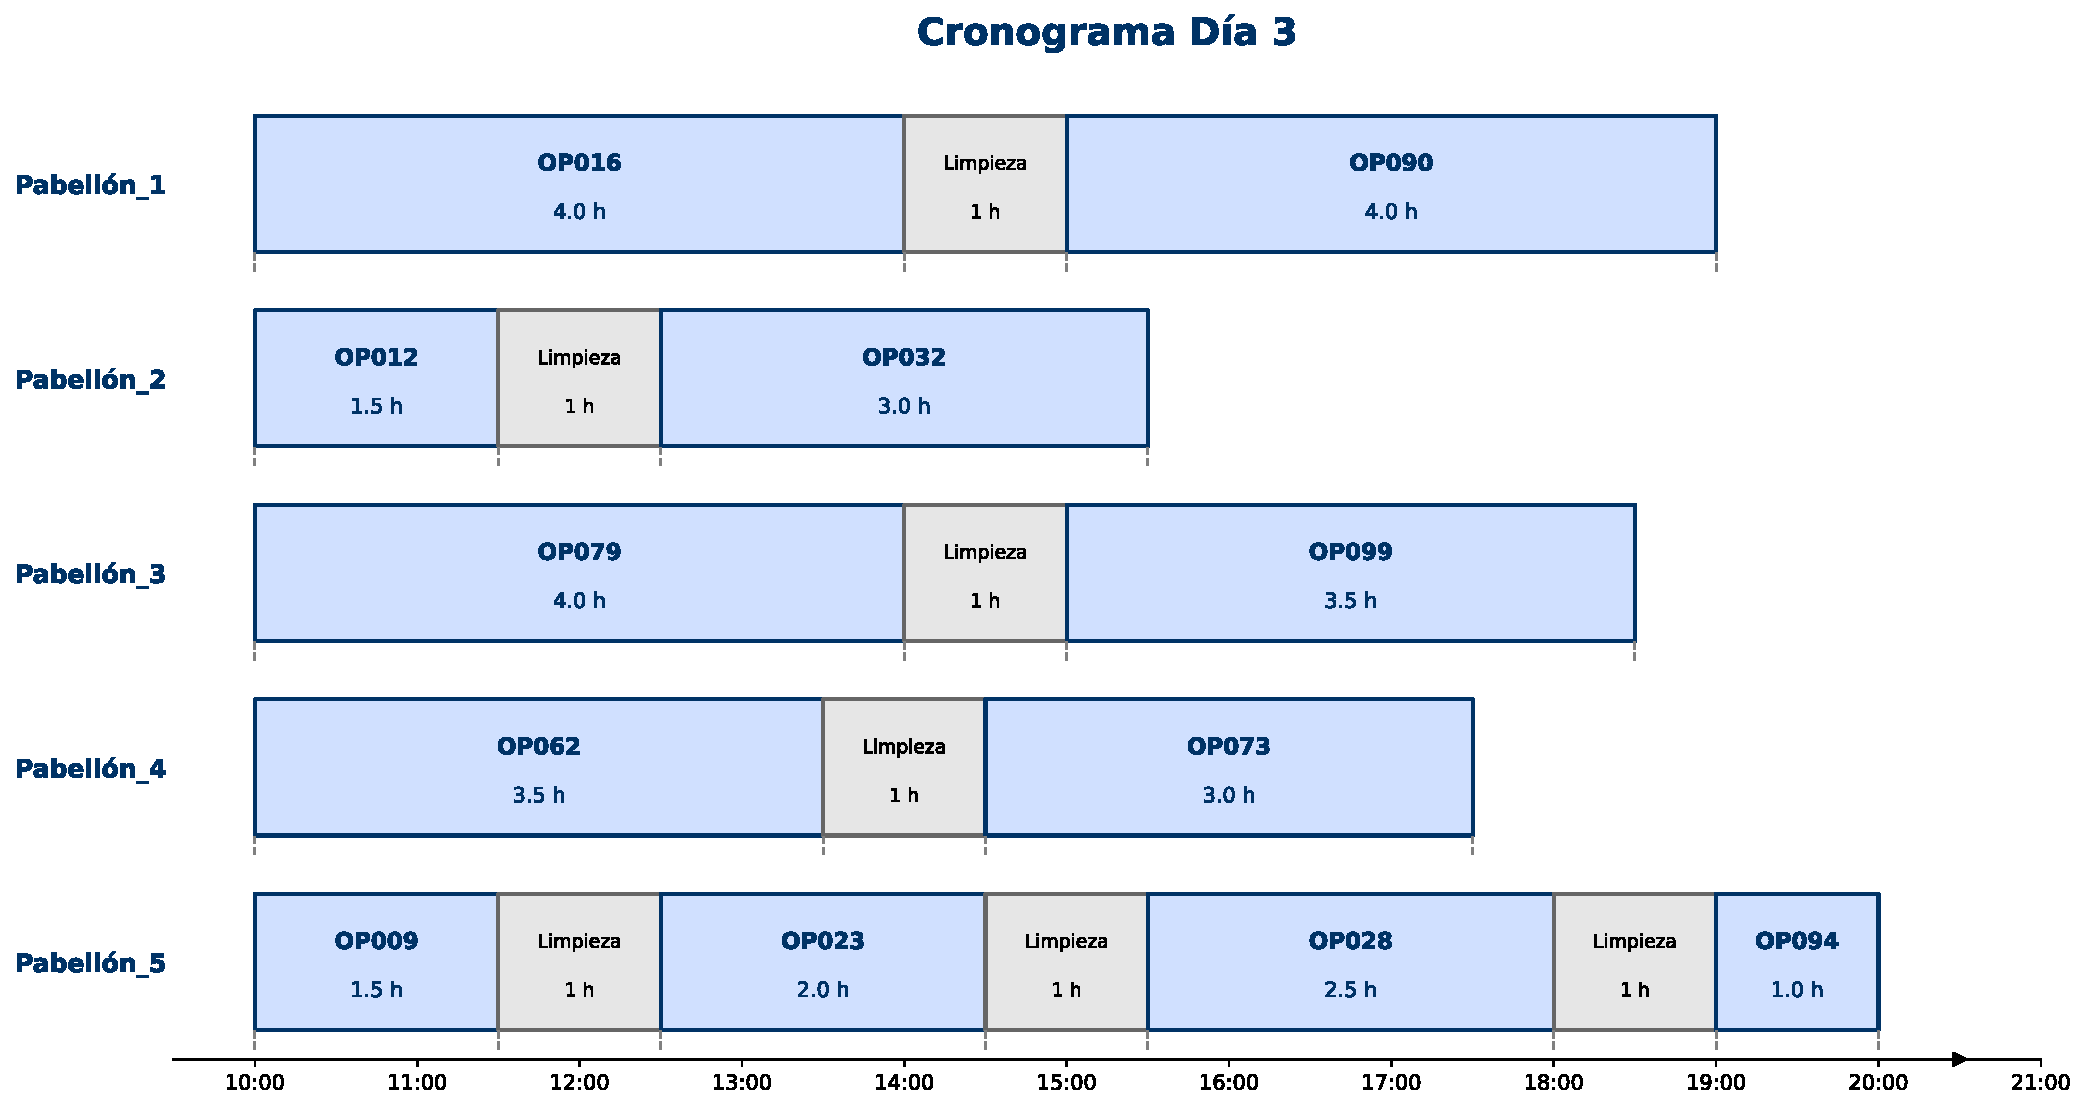
\includegraphics[width=0.8\textwidth]{./TeX_Files/graphs/Cronograma_Dia3.pdf}
		\caption{Cronograma con asignación de operaciones - Día 3.}
		\label{fig:cronograma_dia3}
	\end{figure}
	
	\begin{figure}[htbp]
		\centering
		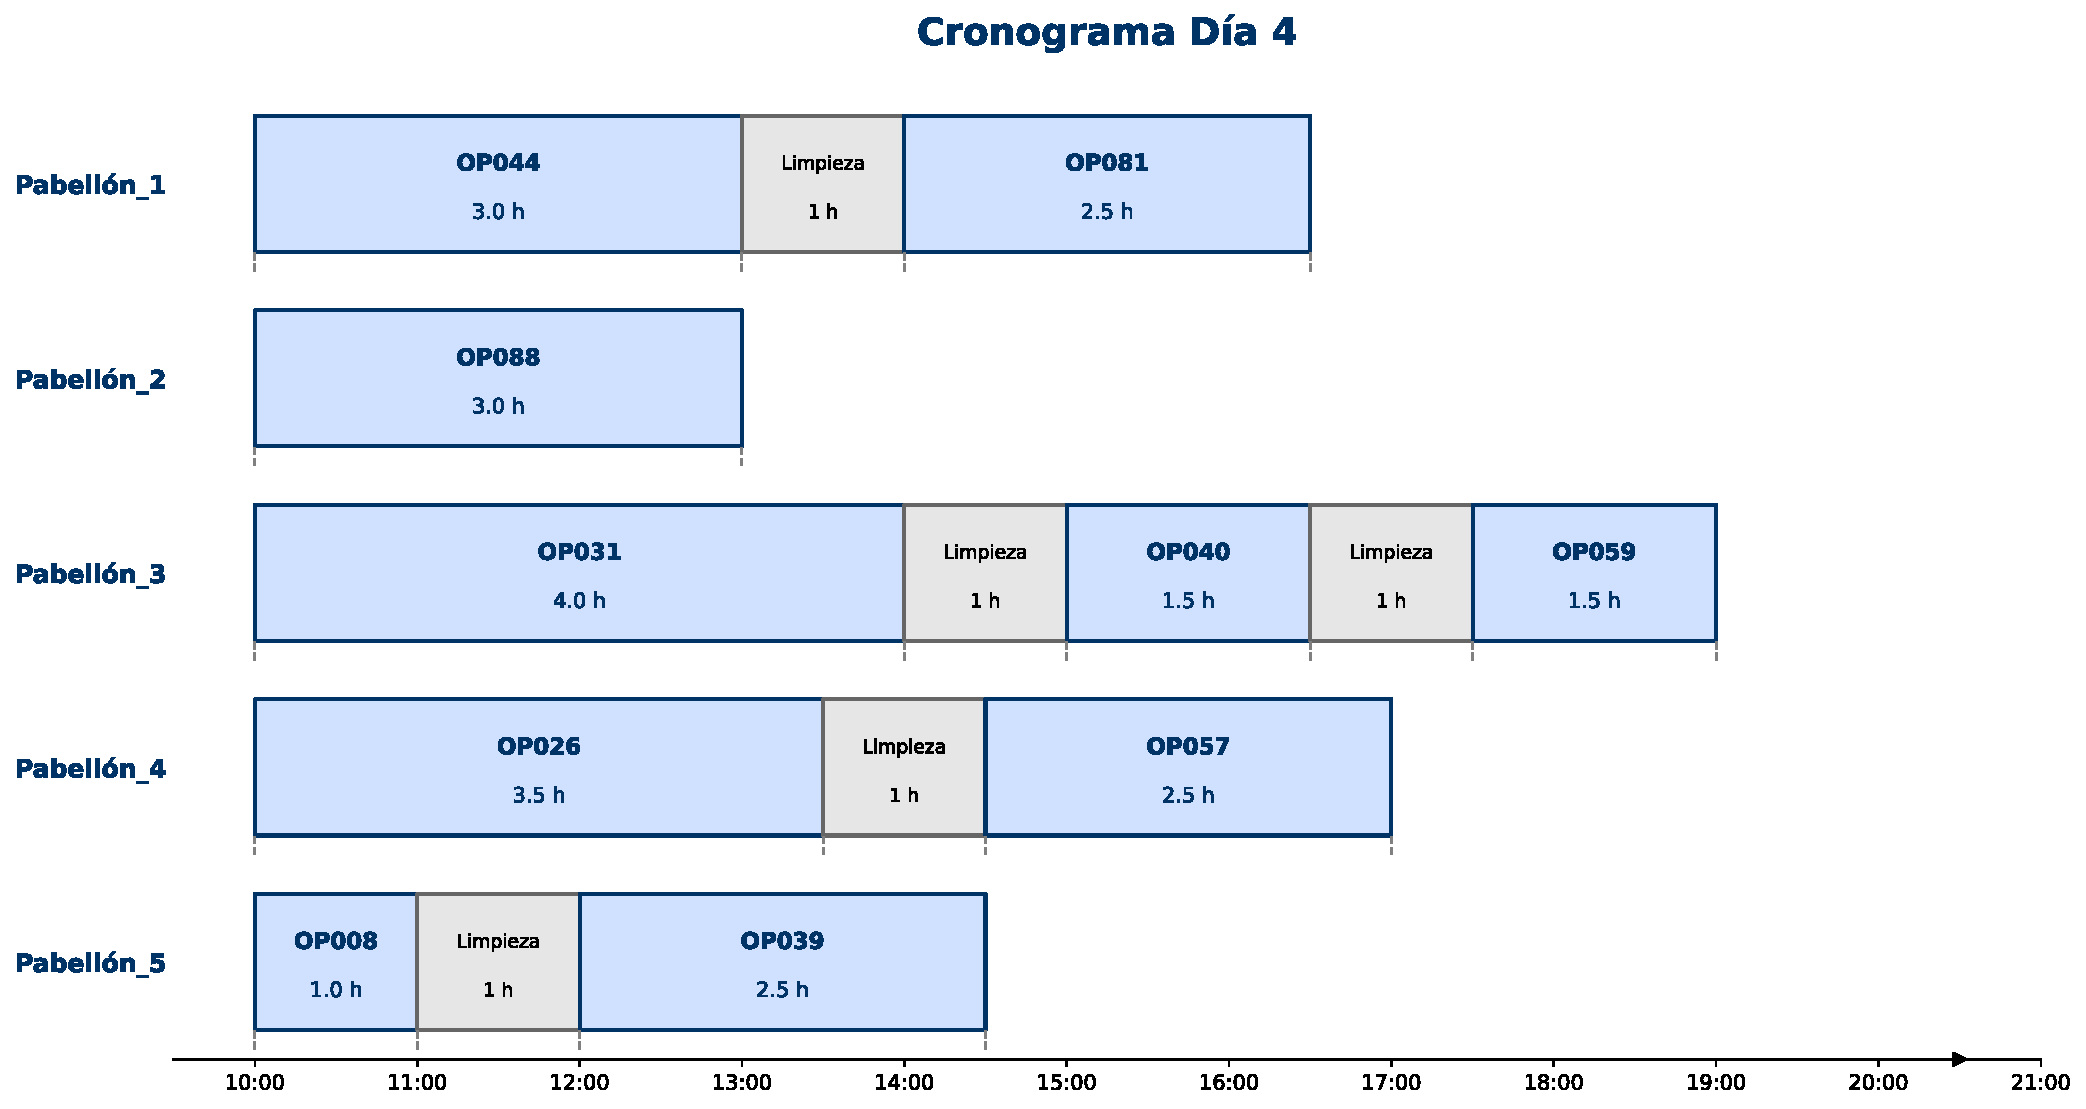
\includegraphics[width=0.8\textwidth]{./TeX_Files/graphs/Cronograma_Dia4.pdf}
		\caption{Cronograma con asignación de operaciones - Día 4.}
		\label{fig:cronograma_dia4}
	\end{figure}
	
	\begin{figure}[htbp]
		\centering
		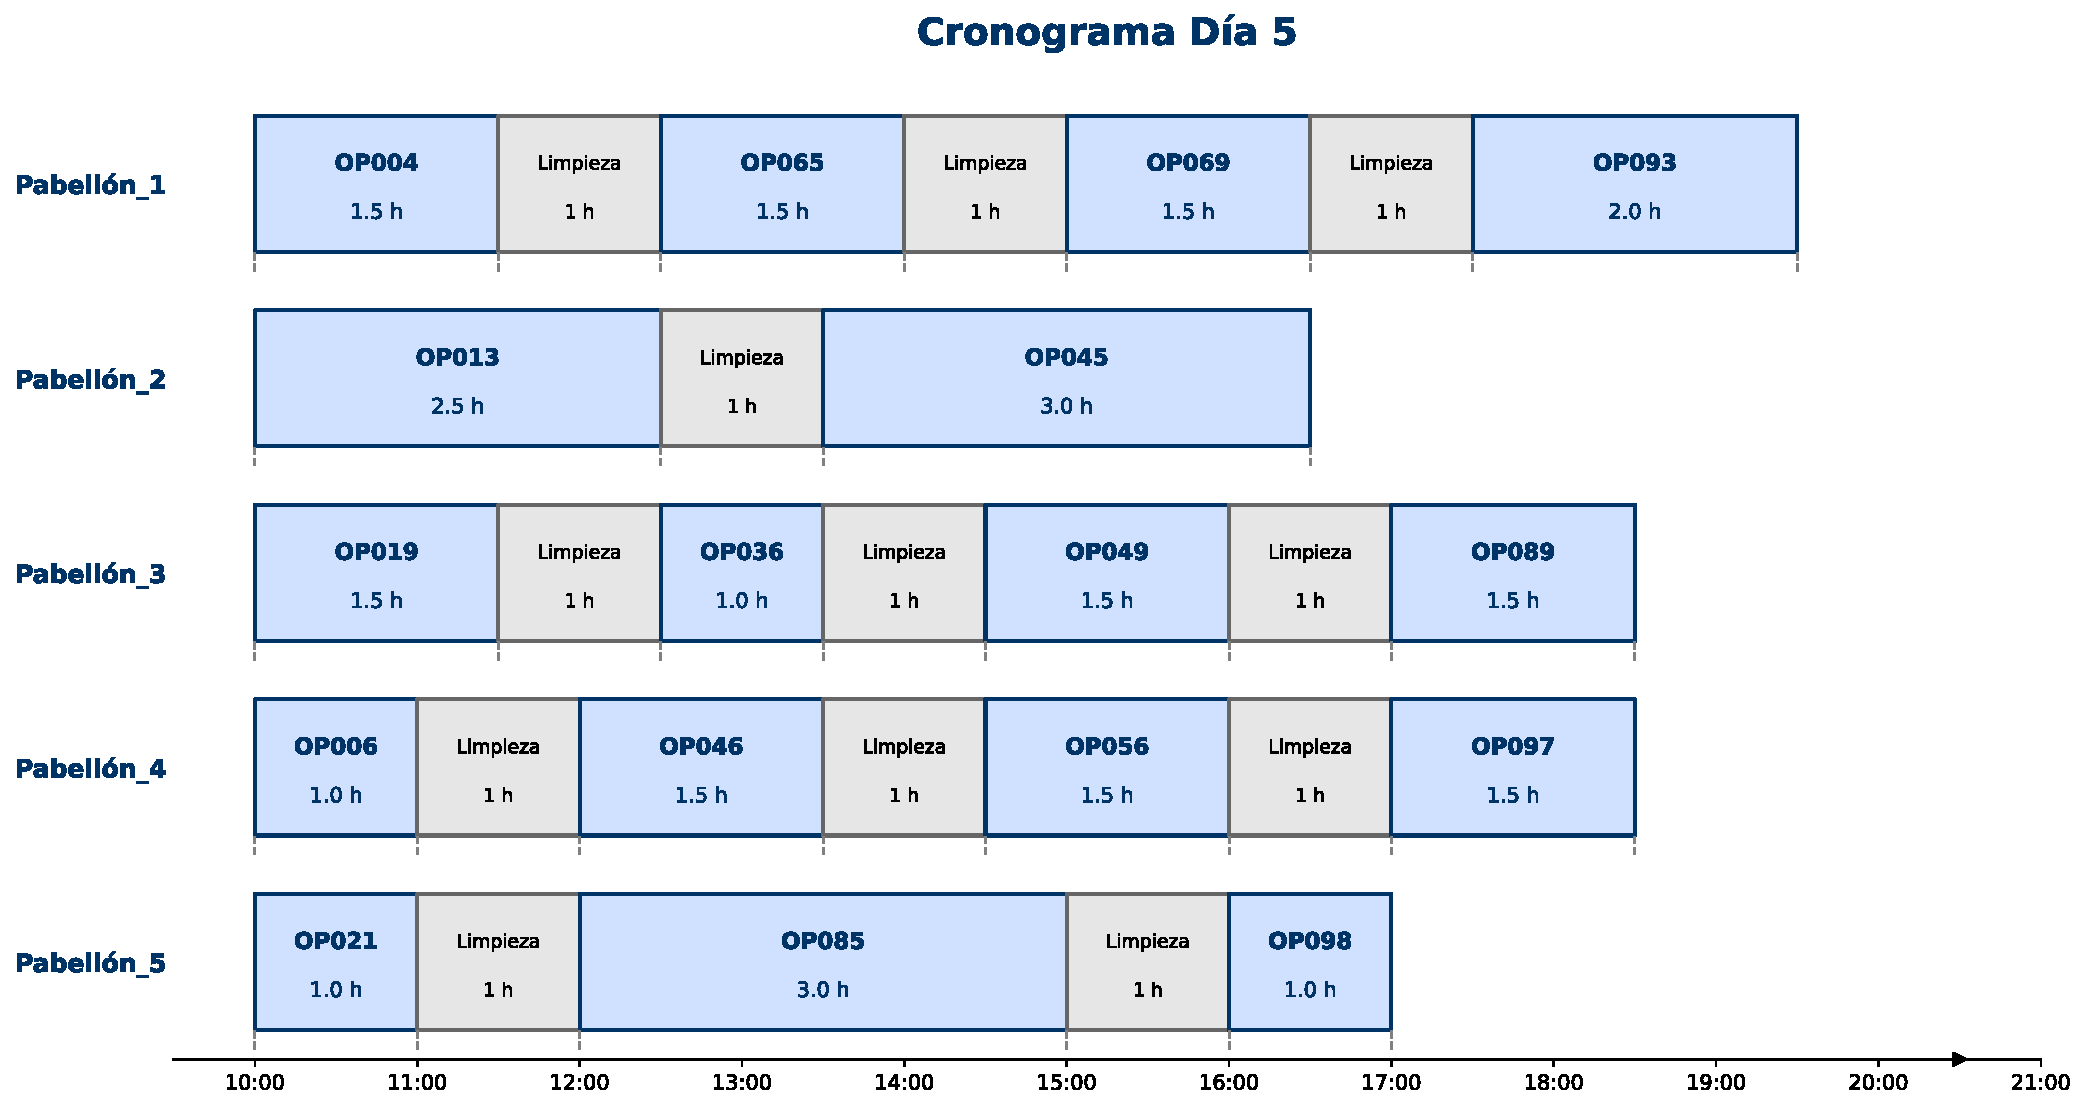
\includegraphics[width=0.8\textwidth]{./TeX_Files/graphs/Cronograma_Dia5.pdf}
		\caption{Cronograma con asignación de operaciones - Día 5.}
		\label{fig:cronograma_dia5}
	\end{figure}
	\clearpage
	
	\section{Modelo C}
	\paragraph{}Siguiendo con el contexto del problema, desde algunos sectores del Ministerio de Salud, se ha planteado la necesidad de cambiar el enfoque del problema, ya que, a juicio de algunos expertos, lo ideal sería poder usar los pabellones la mayor parte del tiempo en operaciones y no en limpiezas.
	Para esto, decidimos plantear una nueva función objetivo para maximizar la suma de las horas asignadas:
	
	$$\max T = \sum_{i\in I} \sum_{j \in J} \sum_{k \in K} X_{i,j,k} t_i$$
	
	Resolvimos el modelo, el cuál nos indicó que el óptimo se encuentra en 152 horas.
	$$T^* = 152$$
	Luego, en base a ese número decidimos ir resolviendo modelos de manera secuencial para obtener la mayor cantidad de operaciones y los costos óptimos. Para ello, agregamos la restricción: 
	
	$$\sum_{i\in I} \sum_{j \in J} \sum_{k \in K} X_{i,j,k} t_i = 152$$
	
	Y modificamos la función objetivo para maximizar la cantidad total de operaciones realizadas:
	
	$$\max Z = \sum_{i\in I} \sum_{j \in J} \sum_{k \in K} X_{i,j,k}$$
	
	Al resolver el modelo, nos entrega un valor óptimo de 53 operaciones
	
	$$Z^* = 53$$
	
	Luego, agregamos este valor como restricción, siguiendo la misma lógica anterior:
	
	$$\sum_{i\in I} \sum_{j \in J} \sum_{k \in K} X_{i,j,k} = 53$$
	
	Finalmente, modificamos la función objetivo para minimizar el costo:
	
	$$\min C = \sum_{i\in I} \sum_{j \in J} \sum_{k \in K} X_{i,j,k} c_i$$
	
	Obteniendo un valor óptimo de \$99.852.714:
	$$C^* = 99.852.714$$
	
	
	\clearpage
	Además, se obtienen los nuevos cronogramas:
		\begin{figure}[htbp]
		\centering
		
\includegraphics[width=0.8\textwidth]{./TeX_Files/graphs/Pregunta_C/Cronograma_Dia1.pdf}
		\caption{Cronograma con asignación de operaciones - Día 1 (Modelo C).}
		\label{fig:cronograma_dia1_modelo_C}
	\end{figure}
	
	\begin{figure}[htbp]
		\centering
		
\includegraphics[width=0.8\textwidth]{./TeX_Files/graphs/Pregunta_C/Cronograma_Dia2.pdf}
		\caption{Cronograma con asignación de operaciones - Día 2 (Modelo C).}
		\label{fig:cronograma_dia2_modelo_C}
	\end{figure}
	
	\begin{figure}[htbp]
		\centering
		
\includegraphics[width=0.8\textwidth]{./TeX_Files/graphs/Pregunta_C/Cronograma_Dia3.pdf}
		\caption{Cronograma con asignación de operaciones - Día 3 (Modelo C).}
		\label{fig:cronograma_dia3_modelo_C}
	\end{figure}
	
	\begin{figure}[htbp]
		\centering
		
\includegraphics[width=0.8\textwidth]{./TeX_Files/graphs/Pregunta_C/Cronograma_Dia4.pdf}
		\caption{Cronograma con asignación de operaciones - Día 4 (Modelo C).}
		\label{fig:cronograma_dia4_modelo_C}
	\end{figure}
	
	\begin{figure}[htbp]
		\centering
		
\includegraphics[width=0.8\textwidth]{./TeX_Files/graphs/Pregunta_C/Cronograma_Dia5.pdf}
		\caption{Cronograma con asignación de operaciones - Día 5 (Modelo C).}
		\label{fig:cronograma_dia5_modelo_C}
	\end{figure}
	\clearpage
	
	
	
	\subsection{Comparación}
	
	\subsubsection*{Comparativa general}
	\begin{table}[htbp]
		\centering
		\caption{Comparativa general de modelos}
		\begin{tabular}{lcc}
			\toprule
			\textbf{Indicador} & \textbf{Modelo B} & \textbf{Modelo C} \\
			\midrule
			Total operaciones & 58 & 53 \\
			Utilización de pabellones & 53,60\% & 60,80\% \\
			Costo total (\$) & 97.802.912 & 99.852.714 \\
			\bottomrule
		\end{tabular}
	\end{table}
	
	El modelo C logra una mejor utilización de los pabellones, logrando un aumento del 7,2\% de utilización (de 53,60\% a 60,80\%). Es más caro, siendo \$2.049.802 mayor que el modelo B. Además, logra 5 operaciones menos en total, con 53 versus 58.
	
	\subsubsection*{Operaciones por día}
	\begin{table}[htbp]
		\centering
		\caption{Operaciones por día}
		\begin{tabular}{ccc}
			\toprule
			\textbf{Día} & \textbf{Modelo B} & \textbf{Modelo C} \\
			\midrule
			1 & 11 & 10 \\
			2 & 8 & 8 \\
			3 & 12 & 12 \\
			4 & 10 & 11 \\
			5 & 17 & 12 \\
			\bottomrule
		\end{tabular}
	\end{table}
	
	El modelo C distribuye de forma más equitativa y similar las operaciones por cada día.
	
	\subsubsection*{Tipos de operaciones}
	\begin{table}[htbp]
		\centering
		\caption{Tipos de operaciones y costos asociados}
		\resizebox{\textwidth}{!}{
		\begin{tabular}{lrrrr}
			\toprule
			\textbf{Tipo de Operación} & \textbf{\% (Modelo B)} & \textbf{Costo (Modelo B)} & \textbf{\% (Modelo C)} & \textbf{Costo (Modelo C)} \\
			\midrule
			Gástrica              & 20,69\% & \$23.540.589 & 11,32\% & \$12.950.361 \\
			Traumatológica        & 13,79\% & \$16.150.372 & 22,64\% & \$33.250.622 \\
			Ginecológica          & 13,79\% & \$13.960.515 & 11,32\% & \$11.380.327 \\
			Vascular              & 3,45\%  & \$4.600.068  & 0,00\%  & \$0 \\
			Dérmica               & 12,07\% & \$8.210.241  & 13,21\% & \$8.210.241 \\
			Urológica             & 3,45\%  & \$4.510.138  & 5,66\%  & \$7.230.174 \\
			Oftalmológica         & 18,97\% & \$14.530.699 & 20,75\% & \$14.530.699 \\
			Otorrinolaringológica & 13,79\% & \$12.300.290 & 15,09\% & \$12.300.290 \\
			\bottomrule
		\end{tabular}
		}
	\end{table}
	
	Acá podemos ver que en el Modelo C no se realiza ninguna operación Vascular, mientras que en el B se hace una. Se hacen más traumatológicas, un 8,85\% más. Se hacen menos en gástrica, un 9,37\% menos.
	
	Al comparar los cronogramas gráficos, podemos ver que el modelo C toma cirugías más largas, a diferencia del B que intenta poner la mayor cantidad de cirugías por lo que favorece a las de menor tiempo. Como cada cirugía independiente de su tiempo tiene que tener una limpieza de 1 hora, hacer varias operaciones cortas requiere mucho tiempo de limpieza que se ``pierde'', en cambio, si es una cirugía larga, se requiere 1 sola limpieza.
	
	El modelo C termina atendiendo 5 pacientes menos, sin embargo, toma más operaciones largas, las cuales por su naturaleza son más graves, por lo que estaría priorizando pacientes de gravedad frente a pacientes que requieren operaciones menores.
	
	En conclusión, decidimos que el modelo C es el más apropiado para el contexto del problema, ya que el país se encuentra en una situación crítica. Para agregar y mejorar el modelo, como vimos antes se había anulado la operación vascular al optimizar, por lo que se podría considerar algunos tipos de operación como más prioritarios al asignarle un peso al tipo.

	\section{Sensibilidad}
	\paragraph{}Desde el Ministerio de Hacienda, han indicado que el presupuesto asignado al programa se encuentra en revisión, por lo cual podría reducirse, mantenerse o incrementarse. Para analizar cómo esto afecta al plan de operaciones, resolvimos el modelo base variando el presupuesto.

	\subsection{Resolución con distintos presupuestos}
	Resolvimos el modelo base con presupuestos que van desde los \$50.000.000 hasta los \$150.000.000, aumentando en \$5.000.000 por cada resolución, lo que nos dio 21 escenarios distintos.

	Para cada nivel de presupuesto, aplicamos la misma resolución secuencial del Modelo B: primero maximizamos la cantidad de operaciones sujeta al nuevo presupuesto, y luego, fijando dicho óptimo como restricción, minimizamos el costo total. Los resultados obtenidos se resumen en la siguiente tabla:

	\begin{table}[htbp]
		\centering
		\caption{Resultados por nivel de presupuesto}
		\label{tab:sensibilidad}
		\begin{tabular}{lcc}
			\toprule
			\textbf{Presupuesto} & \textbf{Operaciones} & \textbf{Costo Mínimo} \\
			\midrule
			\$50.000.000  & 35 & \$48.731.673 \\
			\$55.000.000  & 38 & \$54.041.836 \\
			\$60.000.000  & 41 & \$59.521.967 \\
			\$65.000.000  & 43 & \$63.302.096 \\
			\$70.000.000  & 46 & \$69.532.228 \\
			\$75.000.000  & 48 & \$73.962.359 \\
			\$80.000.000  & 50 & \$78.492.424 \\
			\$85.000.000  & 52 & \$83.182.599 \\
			\$90.000.000  & 54 & \$87.932.675 \\
			\$95.000.000  & 56 & \$92.782.814 \\
			\textbf{\$100.000.000} & \textbf{58} & \textbf{\$97.802.912} \\
			\$105.000.000 & 60 & \$102.892.976 \\
			\$110.000.000 & 62 & \$108.453.088 \\
			\$115.000.000 & 64 & \$114.293.229 \\
			\$120.000.000 & 65 & \$117.253.275 \\
			\$125.000.000 & 67 & \$123.223.411 \\
			\$130.000.000 & 69 & \$129.273.533 \\
			\$135.000.000 & 70 & \$132.393.546 \\
			\$140.000.000 & 72 & \$138.903.593 \\
			\$145.000.000 & 73 & \$142.223.607 \\
			\$150.000.000 & 75 & \$149.163.724 \\
			\bottomrule
		\end{tabular}
	\end{table}
	\clearpage

	La fila resaltada corresponde al presupuesto original de \$100.000.000. Se puede observar que, a medida que el presupuesto aumenta, la cantidad de operaciones realizadas crece de forma consistente, pasando de 35 operaciones con \$50.000.000 hasta 75 operaciones con \$150.000.000.

	\subsection{Gráfico de sensibilidad}
	Graficamos las soluciones obtenidas considerando en el eje X la cantidad de operaciones y en el eje Y el costo total incurrido, como se puede observar en la Figura~\ref{fig:sensibilidad}.

	\begin{figure}[htbp]
		\centering
		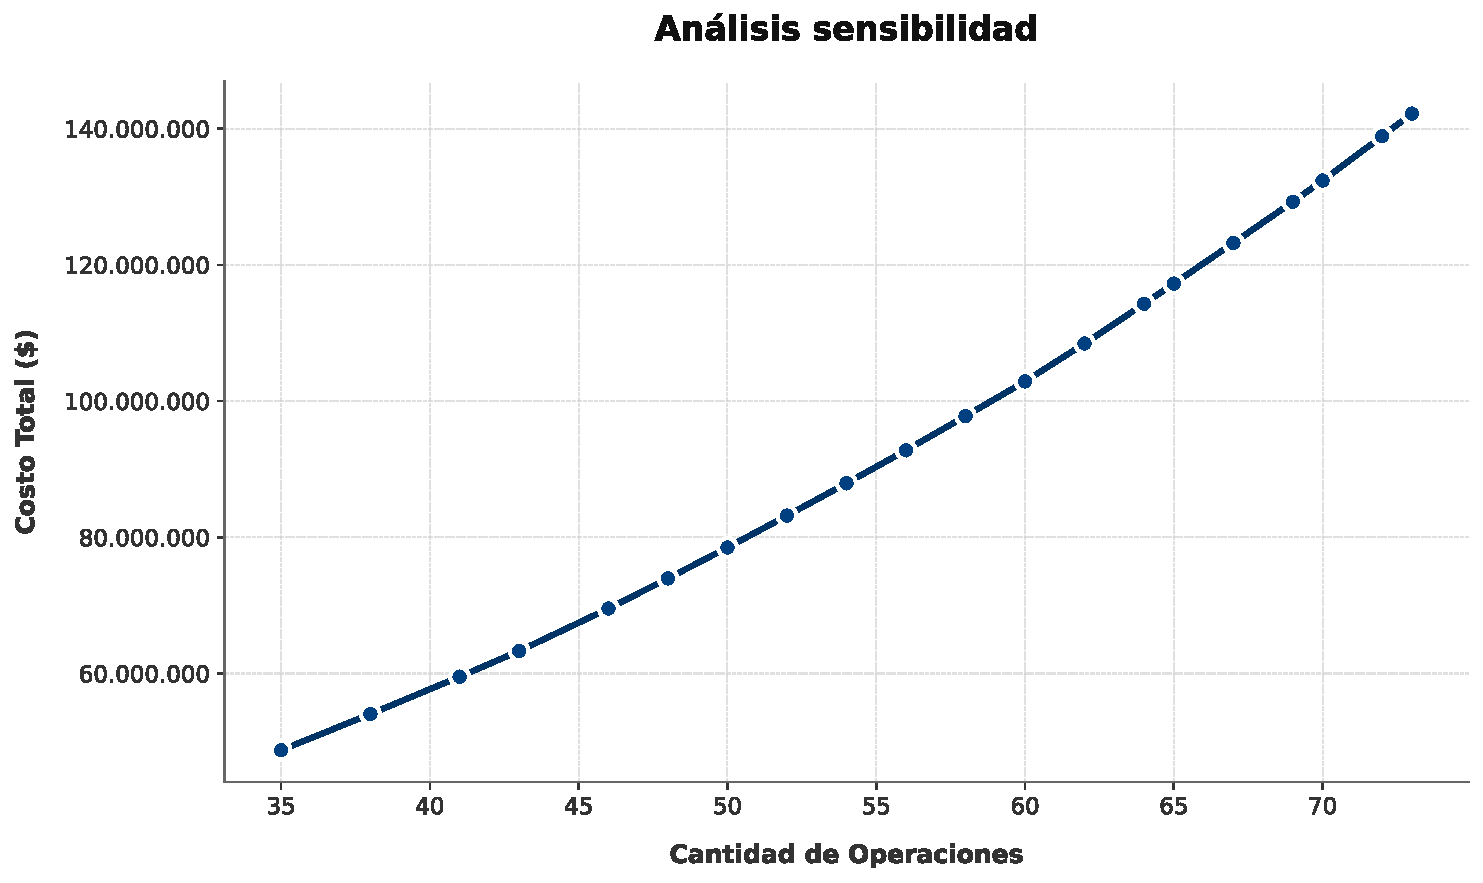
\includegraphics[width=0.85\textwidth]{./TeX_Files/graphs/Sensibilidad_Presupuesto.pdf}
		\caption{Análisis de sensibilidad: cantidad de operaciones vs.\ costo total.}
		\label{fig:sensibilidad}
	\end{figure}

	\subsection{Discusión}
	Del gráfico y la tabla podemos observar que la relación entre la cantidad de operaciones y el costo total es casi lineal. En promedio, por cada \$5.000.000 adicionales de presupuesto se logran realizar aproximadamente 2 operaciones más, lo que indica un costo marginal estable de alrededor de \$2.500.000 por operación adicional. Esto nos indica que, dentro del rango analizado, la eficiencia del gasto se mantiene consistente: no hay retornos decrecientes significativos ni saltos abruptos en la curva.

	Si el presupuesto se redujera a la mitad (\$50.000.000), el modelo aún logra realizar 35 operaciones, lo que representa un 60,3\% de las 58 operaciones originales. Por otro lado, si se dispusiera de un incremento modesto de \$10.000.000 (llegando a \$110.000.000), se podrían realizar 62 operaciones, es decir, 4 más que con el presupuesto actual.
	
	\chapter{Conclusión}
	
	El presente proyecto abordó el problema de planificación de cirugías electivas para el contingente de salud que visitará el Hospital Regional de Villa Zarcillo durante la semana del 6 de julio, mediante la formulación y resolución de modelos de programación lineal entera.
	
	En primer lugar, el modelo base (Modelo B), orientado a maximizar la cantidad de operaciones realizadas sujeto a un presupuesto de \$100.000.000, permitió atender a 58 pacientes con un costo de \$97.802.912 y una utilización promedio de los pabellones de 53,60\%. Este resultado evidenció que, si bien el objetivo principal, maximizar pacientes atendidos, se cumple satisfactoriamente, el uso del tiempo disponible en los pabellones queda lejos de su capacidad máxima, principalmente debido a la fragmentación del tiempo en limpiezas asociadas a operaciones de corta duración.
	
	Frente a esto, el Modelo C propuso un enfoque alternativo, maximizando el porcentaje de uso de los pabellones. Esta variante logró elevar la utilización a 60,80\%, priorizando cirugías de mayor duración y, por ende, de mayor complejidad clínica. Sin embargo, este enfoque implicó atender a 5 pacientes menos (53 versus 58) y un costo levemente superior (\$99.852.714), además de eliminar por completo las operaciones de tipo vascular. Al comparar ambos enfoques, se concluyó que el Modelo C resulta más adecuado para el contexto de crisis sanitaria descrito, dado que prioriza a los pacientes con operaciones más graves por sobre la cantidad total de operaciones, aunque se identificó como oportunidad de mejora la incorporación de ponderadores por tipo de operación, de manera de evitar la exclusión completa de alguna especialidad.
	
	Por otra parte, el análisis de sensibilidad sobre el presupuesto, realizado para el Modelo B en un rango de \$50.000.000 a \$150.000.000, mostró una relación prácticamente lineal entre el presupuesto disponible y la cantidad de operaciones realizadas, con un costo marginal estable cercano a \$2.500.000 por operación adicional. Esto indica que, dentro del rango estudiado, no existen retornos decrecientes ni umbrales críticos: cualquier variación en el presupuesto asignado se traduce de manera proporcional en la cantidad de pacientes que pueden ser atendidos, sin que la restricción de tiempo disponible en los pabellones llegue a ser el factor limitante.
	
	En síntesis, el uso de herramientas de optimización permitió no solo determinar una planificación factible y eficiente para el contingente de salud, sino también comparar distintos criterios de priorización (cantidad de pacientes versus uso de la infraestructura) y cuantificar el impacto de decisiones presupuestarias externas sobre la capacidad de respuesta del sistema. Como trabajo futuro, se sugiere explorar modelos que incorporen explícitamente la gravedad o urgencia de cada operación como parámetro de ponderación, así como evaluar escenarios con disponibilidad variable de pabellones a lo largo de la semana.


\begin{thebibliography}{9}
	\bibitem{clases} Acuña, J., Ph.D. (2026).
	\emph{Apuntes de clases, ING200 Optimización}.
	Primer semestre 2026. Universidad Adolfo Ibáñez, Viña del Mar, Chile.
\end{thebibliography}
\end{document}